\documentclass{article}

% Language setting
% Replace `english' with e.g. `spanish' to change the document language
\usepackage[english]{babel}

% Set page size and margins
% Replace `letterpaper' with `a4paper' for UK/EU standard size
\usepackage[a4paper,top=2cm,bottom=2cm,left=3cm,right=3cm,marginparwidth=1.75cm]{geometry}

% Useful packages
\usepackage{amsmath}
\DeclareMathOperator{\sinc}{sinc}
\DeclareMathOperator*{\argmax}{arg\,max}
\DeclareMathOperator*{\argmin}{arg\,min}

\usepackage{amssymb}
\usepackage{float}
\usepackage{graphicx}
\usepackage[colorlinks=true, allcolors=blue]{hyperref}

\usepackage{tikz}
\usetikzlibrary{arrows,decorations.pathmorphing,backgrounds,fit,positioning,shapes.symbols,chains,shapes.geometric,shapes.arrows,calc}

\usepackage{listings}
\usepackage{xcolor}
\usepackage{enumitem}
\usepackage{physics}
\setlist[itemize]{nosep}

\definecolor{codegreen}{rgb}{0,0.6,0}
\definecolor{codegray}{rgb}{0.5,0.5,0.5}
\definecolor{codepurple}{rgb}{0.58,0,0.82}
\definecolor{backcolour}{rgb}{0.95,0.95,0.92}

\lstdefinestyle{mystyle}{
  backgroundcolor=\color{backcolour},
  commentstyle=\color{codegreen},
  keywordstyle=\color{magenta},
  numberstyle=\tiny\color{codegray},
  stringstyle=\color{codepurple},
  basicstyle=\ttfamily\footnotesize,
  breakatwhitespace=false,
  breaklines=true,
  captionpos=b,
  keepspaces=true,
  numbers=left,
  numbersep=5pt,
  showspaces=false,
  showstringspaces=false,
  showtabs=false,
  tabsize=2
}

\lstset{style=mystyle}

\title{Computational Imaging}
\author{Matteo Galiazzo}

\begin{document}

\maketitle

\tableofcontents

\section{Introduction}

Image processing is the field of enhancing the images by tuning many parameters and features of the images.
Image processing is the subset of computer vision.
Here, transformations are applied to an input image and the resultant output image is returned.
In computer vision we extract insights from images and videos, input can be both image and video, and the output can be an interpretation, which is often non-visual.
In image processing input and output are both images, and the operations are at low-level and affect pixels within the image.

A continuous image is a function $f:\omega \in \mathbb{R}^2 \rightarrow R$.
A discrete image $A$ is a matrix of size $M \times N$ obtained by discretizing the function f.
The intersection between a row and a column is called pixel.
The value assigned to every pixel is the average brightness in the pixel rounded to the nearest integer value.
The process of representing the amplitude of the $2D$ signal at a given coordinate as an integer value with $L$ different gray levels is usually referred to as amplitude quantization.

Many techniques developed for the single channel image are repeated on the three channels.
Different manipulating operations can be performed on the images, such as:
\begin{itemize}
  \item Transforming the color space.
  \item Applying fine transformations.
  \item Create cartoonized images.
  \item Object detection using colors in HSV.
\end{itemize}

Computational algorithms are essential to convert data to images, since sensors almost never directly generate usable images.

The reconstruction algorithm necessarily requires the solution of an inverse problem.
We call two problems inverse one another if the formulation of the each involves part or all the formulation of the other.
The problem that is more extensively studied is usually called forward (or direct), the other is called inverse.
The direct problem is usually oriented along a cause-effect, in the sense that it computes the effect given the cause.
The inverse problem is associated with the reversal of the cause-effect and consists in finding the causes given the effects.
In direct problems usually there is a loss of information from the input to the output.
Hence, in the solution of the inverse problem it is impossible to recover the object exactly, due to the information lost in the direct one.

Linear inverse imaging problems are characterized by a linear model describing the relationship between the measured data $y$ and the unknown object $x$.
The direct linear model can be expressed as: $Ax = y$, where $A$ is a matrix representing the linear operator acting on the image $x$ to generate the data $y$.
The data $y$ are usually affected by noise, due to different physical processes.
For the moment, we can consider addittive noise so that the final linear model is: $Ax = y+e$.
This is the model we want to invert.
The noise is a random process described by a random variable.
Different random processes can corrupt the data $y$, represented by random variables with different probability distributions.

Digital images are always affected by noise, which is due to:
\begin{itemize}
  \item False light, defects in the recording process.
  \item Quantization error.
  \item Gaussian noise, generated during the conversion of the light to a signal (we will mainly deal with this noise).
  \item Poisson noise, generated due to the discrete nature of electric charges.
\end{itemize}

\textbf{We only have statistical information about the noise}, since we can't sample it.

\section{Ill-posed problems}

Our model is $Ax=y+e$, if we want to invert the model we get an ill-posed problem.
A problem is defined well-posed if:
\begin{enumerate}
  \item It exists a solution for arbitrary data.
  \item This solution is unique.
  \item The solution continuously depends on the data.
\end{enumerate}

% lesson 2
% ill-posed problems (10/22)
This means that \textbf{it small varies for small variations of the data}.
An ill-posed problem happens when at least one of the three conditions is not satisfied.

Linear inverse imaging problems are ill-posed due to noise, since we can't reverse 2 identical problems and get the same solution.

$A$ is a linear operator mapping an image in the image space $X$ to a noise free image in the image space $Y$.
The set of noise free images is usually called range of $A$.

Solving the linear system $Ax = y + e$ is quite a simple numerical task.
Suppose $A$ of size $m \times n$
\begin{itemize}
  \item If $m=n$ and $A$ non singular, the system has a unique solution, but usuallly there is no continuous dependence from the data.
  \item If $m>n$ the linear system has no solution and in place of it we solve the least square problem: $\min || Ax - (y + e) ||^2_2$.
  \item If $m<n$ the system has infinite possible solutions.
\end{itemize}

\textbf{The result is that the numerical inversion produces results that are physically unacceptable even if they are mathematically acceptable}.

In inverse problems data are always affected by noise and the solution method amplifies that noise, producing a large oscillating function that completely hides the physical solution.
So even if the solution of the linear system exists and is unique it is completely corrupted due to the small noise on the data (ill-conditioned system).
\begin{itemize}
  \item case of $A$ square ($m=n$): $A^{-1} y + A^{-1} e = x + A^{-1} e$
  \item case of $A$ rectangular ($m>n$ or $m<n$): $x_{naive} = \min || Ax - (y + e) ||^2_2$
\end{itemize}

The naive image consists of the sum of two images: the first component $x$ is the exact image, the second component $A^{-1} e$ is the inverted noise.

\textbf{The inverted noise contaminates the exact image $x$}.

We can use Singular Value Decomposition of $A$ to analyse the contribution of the inverted noise.
The theorem of singular value decomposition says that any matrix $A$ of size $m\times n$ and rank $k$ can be decomposed as $A = U\sum V^T$.
Where:
\begin{itemize}
  \item $U$ is an orthogonal matrix of size $m\times m$.
  \item $V$ is an orthogonal matrix of size $n\times n$.
  \item $\sum$ is a diagonal matrix with diagonal entries: $\sigma_1 \leq ... \leq \sigma_k \leq 0$.
\end{itemize}

If we write in terms of SVD representation, the naive solution can be written as:

$$x_{naive} = A^{-1} (y+e) = x + A^{-1} e = x + \sum_{i=1}^k \frac{1}{\sigma_i} v_i u_i^T e$$

The error components $|u_i^T e|$ are small and typically of the same order of magnitude for all $i$.
The singular values decay to a value very close to zero.
The singular vectors corresponding to the smaller singluar values typically tend to have more sign changes.

When we divide by a small singular value we greatly magnify the corresponding error component, which contributes a large multiple of the high frequency information contained in the solution.

\begin{figure}[htbp]
  \centering
  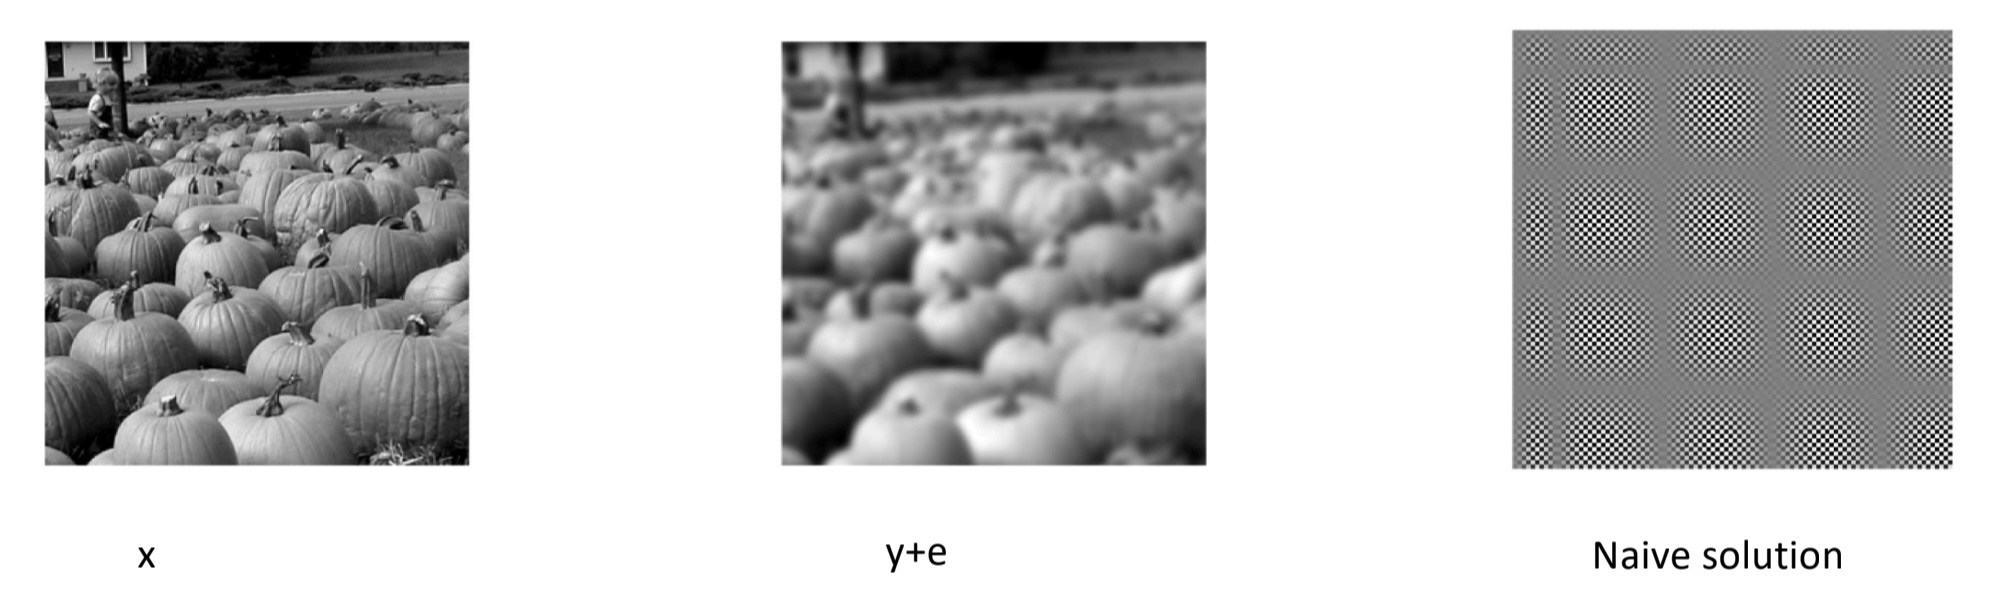
\includegraphics[width=0.7\linewidth]{./img/illposed_noise.jpg}
  \caption{In the presence of errors on the data the solution is dominated by noise}
  \label{fig:illposed_noise}
\end{figure}

\section{Model-based reconstruction methods}

\subsection{Direct regularization}

We introduce a mathematical model to solve the problem.
Direct regularization methods compute the solution of an ill posed inverse problem (imaging) by imposing some costraints on the solution.
The model-based approach mathematically models the problem to be solved as a minimization problem with two acting functions:
\begin{itemize}
  \item The term $||Ax - (y +e)||^2_2$, representing the data fitting.
  \item The regularization term $R(x)$ that incorporates a priori information on the solution.
\end{itemize}

The minimization can be expressed as a constrained minimization or as an equivalent unconstrained minimization $\min || Ax - (y+e)||^2_2 + \lambda R(x)$ where $\lambda$ is the regularization parameter representing the trade off between the fit-to-data and the regularization terms.

\subsection{p-norm regularization}

$R(x) = ||Lx||^p_p$ with $0<p\leq 2$ where the p-norm is defined as $||x||^p_p = (\sum_{i=1}^n x_i^p)^{1/p}$

\subsection{The gradient of an image}
Given a differentiable function $f:\mathbb{R}^2 \rightarrow \mathbb{R}$, we know that the gradient of $f$ is $\nabla f : \mathbb{R}^2 \rightarrow \mathbb{R}^2$ is a function constituted by the partial derivatives of f:
$$\nabla f(x) = (\frac{\partial f}{\partial x_1}, \frac{\partial f}{\partial x_2})^T$$
We remark that if all the partial derivatives of a function $f:\mathbb{R}^n \rightarrow \mathbb{R}$ exist and are continuous in a point $x_0$ then f is said differentiable in $x_0$.
However, the image is not a function, but a matrix. How can we define the gradient of an image?
We consider the discretization of the gradient function and apply it to the pixels of the image.

\begin{figure}[htbp]
  \centering
  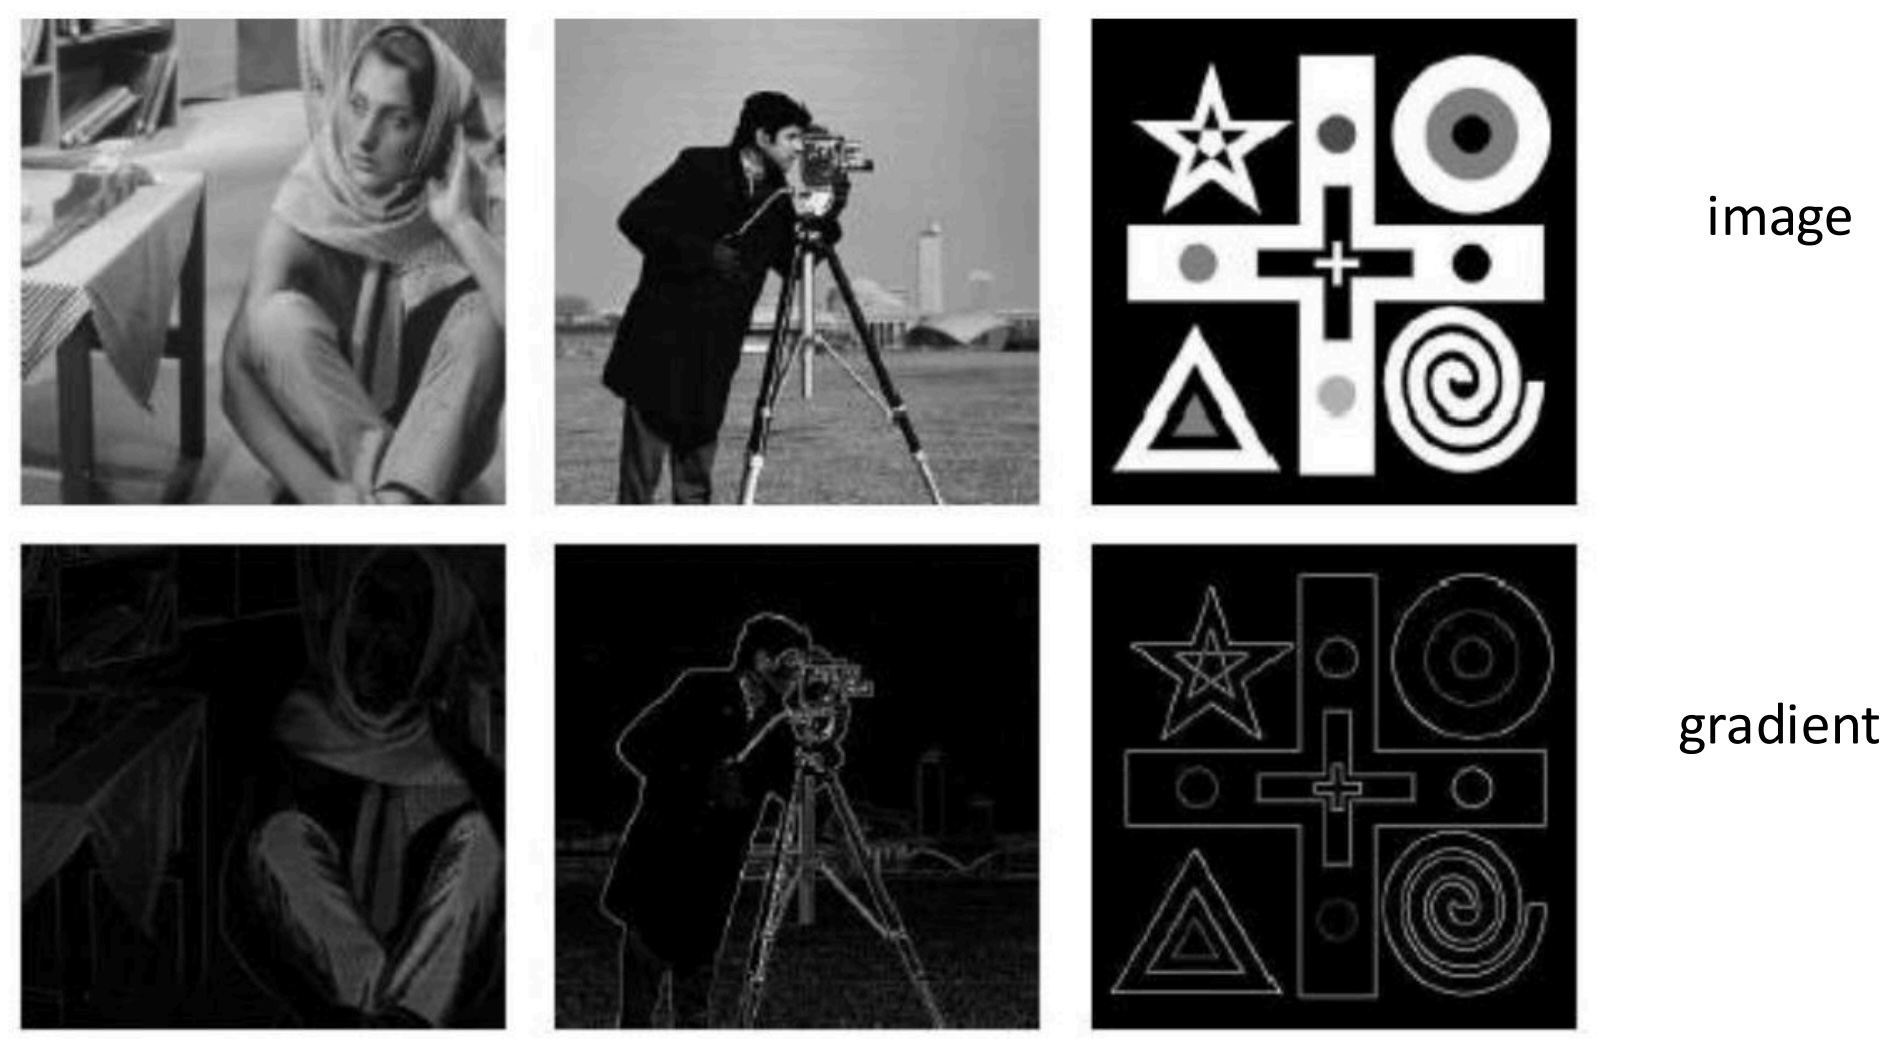
\includegraphics[width=0.7\linewidth]{./img/image_gradient.jpg}
  \caption{The gradients of some images}
  \label{fig:image_gradient}
\end{figure}








\end{document}
